%%%%%%%%%%%%%%%%%%%%%%%%%%%%%%%%%%%%%%%%%%%%%%%%%%%%%%%%%%%%%%%%%%%%%%%%%%%%%%%
%                                                                             %
%           TEMPLATE LATEX PER TESI                                           %
%           ______________                                                    %
%                                                                             %
%           Ultima revisione: 30 Novembre 2023                                %
%           Revisori: G.Presti; L.A.Ludovico; F. Avanzini; M. Tiraboschi      %
%                                                                             %
%%%%%%%%%%%%%%%%%%%%%%%%%%%%%%%%%%%%%%%%%%%%%%%%%%%%%%%%%%%%%%%%%%%%%%%%%%%%%%%

\documentclass[12pt]{report}

% --- PREAMBOLO ---------------------------------------------------------------
% Inserire qui eventuali package da includere o 
% definizioni di comandi personalizzati

% --- PREAMBOLO ---------------------------------------------------------------

% Selezione lingua
\usepackage[italian]{babel}

% Seleziona il font che preferisci lasciando commentata una sola delle seguenti righe:
%\usepackage[defaultfont]{tesi}
\usepackage{tesi}

% INFORMAZIONI SULLA TESI DA COMPILARE!
%   UNIVERSITA' E CORSO DI LAUREA
\university{Universit\`a degli Studi di Milano}
\unilogo{immagini/unimi}
\faculty{Facolt\`a di Scienze e Tecnologie}
\department{Dipartimento di Informatica\\Giovanni Degli Antoni}
\cdl{Corso di Laurea Triennale in\\Informatica Musicale}

%   TITOLO TESI:
\title{Un Template \LaTeX{} per Elaborati\\Triennali o Tesi Magistrali}

%   AUTORE:
\author{Marco Tiraboschi}
\matricola{123456}
% Elaborato Finale per i CdL triennali
% Tesi di Laurea per i CdL magistrali
\typeofthesis{Elaborato Finale}

%   RELATORE E CORRELATORE:
\relatore{Prof. Luca Andrea Ludovico}
\correlatore{Prof. Federico Avanzini}
\correlatore{Prof. Giorgio Presti}

%   ANNO ACCADEMICO
% \the\year inserisce l'anno corrente, per specificare manualmente un anno accademico NON inserire nel formato 1970-1971, ma inserire solo 1970
\academicyear{\the\year} 

%   INDICI
% elenco delle figure (facoltativo)
% \figurespagetrue
% elenco delle tabelle (facoltativo)
% \tablespagetrue

\begin{document}

% Creazione automatica del frontespizio
\makefrontpage
\beforepreface

% 
%			PAGINA DI DEDICA E/O CITAZIONE
%			facoltativa, questa è l'unica cosa che dovete formattare a mano, un po' come vi pare
%

{\raggedleft \large \sl Questo lavoro \`{e} dedicato ai miei genitori\\
	
	\vspace{2cm}
	
	``What I cannot create, I do not understand''
	
	\bigskip
	
	\--- Richard Feynman\\
  
	\vspace{2cm}
	
	``It's not only powerful,\\but it's also inadequate''
	
	\bigskip
	
	\--- Miller Puckette\\}
         
% 
%			PREFAZIONE (facoltativa)
%

% \prefacesection{Prefazione}
% Le prefazioni non sono molto comuni, tuttavia a volte capita che qualcuno voglia dire qualcosa che esuli dal lavoro in s\'e (come un meta-commento sull'elaborato), o voglia fornire informazioni riguardanti l'eventuale progetto entro cui la tesi si colloca (in questo caso \`e probabile che sia il relatore a scrivere questa parte).

%
%			RINGRAZIAMENTI (facoltativi)
%

\prefacesection{Ringraziamenti}
Questa sezione, facoltativa, contiene i ringraziamenti.

%
%			Creazione automatica dell'indice
%

\afterpreface

% 
%			CAPITOLO 1: Introduzione o Abstract
% 

\chapter{Introduzione}
\label{cap:introduzione}

Questo documento ha una duplice funzione: da un lato mostra un esempio completo di tesi redatto in \LaTeX\ e conforme allo standard PDF/A, e dall'altro contiene suggerimenti e risposte a domande frequenti poste dagli studenti. Se ne raccomanda, pertanto, un'attenta lettura.

\section{Il template}
Se questo documento è stato ottenuto tramite condivisione diretta di file, è consigliabile accedere alla versione continuamente aggiornata e disponibile su Overleaf. \begin{center}
    \url{https://www.overleaf.com/read/hmffzxzhhdqn}
\end{center}

Questo template è stato sviluppato, negli anni, dai membri del Laboratorio di Informatica Musicale dell'Università degli Studi di Milano, in particolare da: Giorgio Presti, Luca Andrea Ludovico, Federico Avanzini, e Marco Tiraboschi.

È principalmente inteso per gli elaborati finali del corso di laurea triennale in Informatica Musicale, ma può essere riadattato anche per altri corsi cambiando i metadati nel preambolo. Nel resto del documento, dove non specificato, useremo il termine \textit{tesi} nella sua accezione generica che include anche gli elaborati triennali.

\section{I contenuti}
\label{sec:contenuti}

In generale, gli elaborati di Informatica musicale sono fortemente interdisciplinari. \`{E} però fondamentale ricordarsi che si tratta di lavori in area informatica, e questo aspetto deve emergere con chiarezza. Anche gli elaborati di contenuto più umanistico devono mostrare rigore scientifico e uno sforzo di formalizzazione nel loro svolgimento. In concreto, sono molto apprezzati schemi, tabelle, formalismi grafici e/o matematici, presenza di parti significative di codice (ove possibile).

Uno scritto di questa estensione parte sempre da un punto pregresso, tipicamente l'analisi dello stato dell'arte e della letteratura. \`{E} poi richiesto un contributo personale (e originale, nel caso delle tesi magistrali) per giungere a una conclusione formulata dall'autore, eventualmente anche in contrasto con il pensiero corrente o con quanto ci si prefigge all'inizio dell'opera.

Le tre fasi devono emergere con chiarezza:
\begin{itemize}
	\item analisi dello stato dell'arte e/o della letteratura;
	\item contributo personale alla ricerca;
	\item conclusioni raggiunte, ed eventuali sviluppi futuri.
\end{itemize}

Nel loro complesso queste tre componenti devono rendere evidente la {\em rilevanza} del lavoro, in termini di
\begin{itemize}
\item chiarezza nella definizione del problema, delle motivazioni e degli obiettivi della tesi; 
\item connessione con la letteratura (cos\`i da mostrare che la tematica oggetto della tesi \`e di interesse per la comunit\`a scientifica);
\item rilevanza della tematica nell'ambito delle discipline informatiche.
\end{itemize}


\section{Organizzazione della tesi}
\label{sec:organizzazione}

La scelta di come strutturare un lavoro esteso, quale un elaborato finale o una tesi, non è semplice n\`{e} univoca, pertanto quelli sotto elencati vanno presi come suggerimenti generici e attualizzati alla propria situazione personale.

\begin{figure}[t]
	\centering
	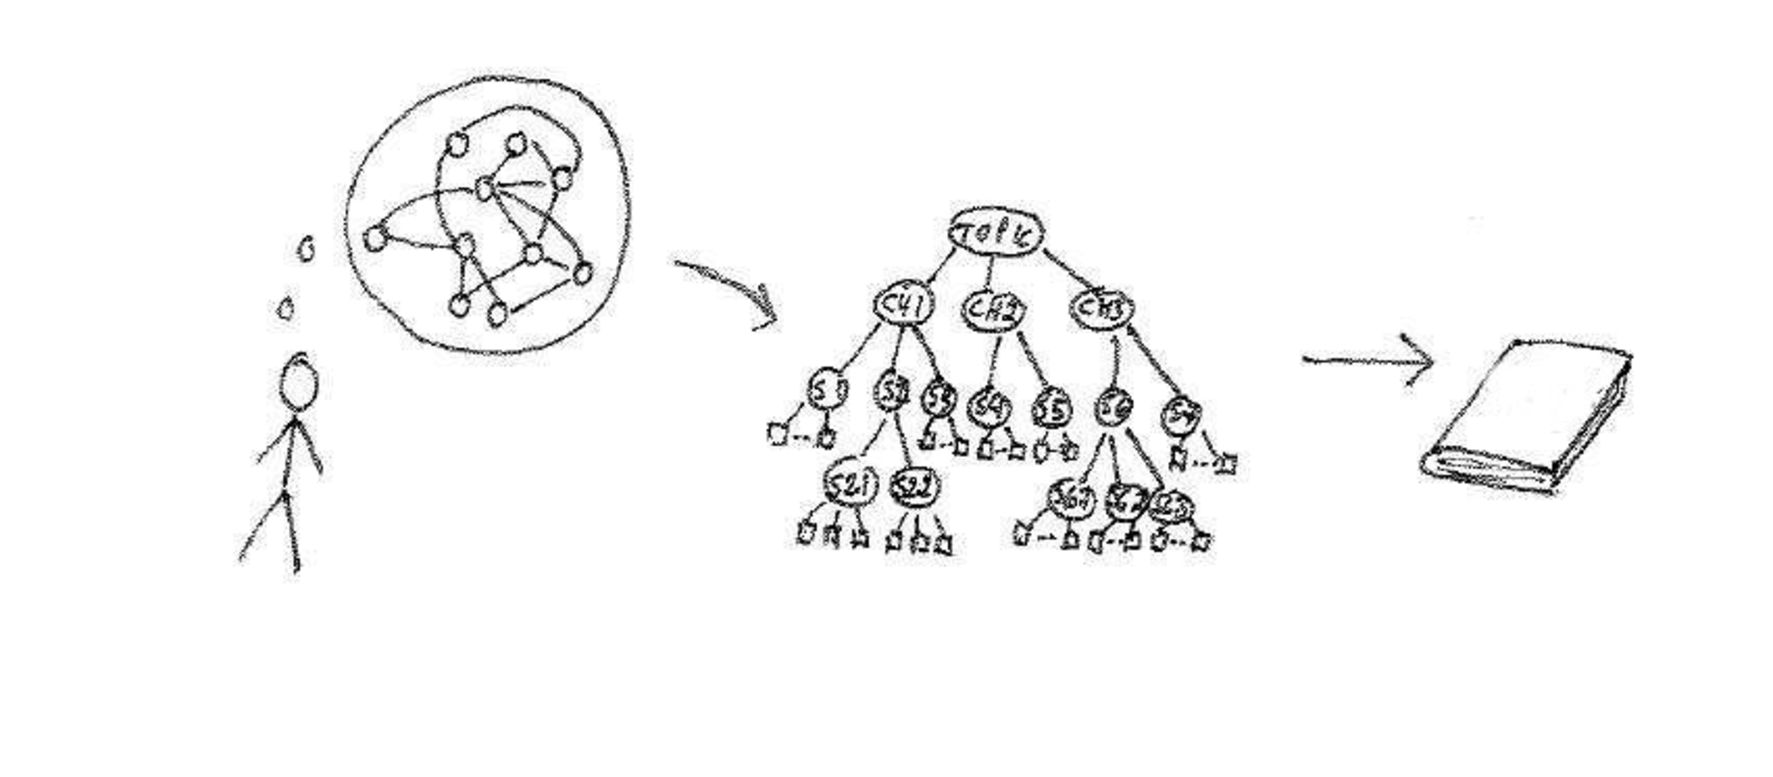
\includegraphics[width = 150mm, trim={0 25mm 0 0}, clip]{immagini/ideas2text}
	\caption{Il processo di trasformazione delle idee in testo~\cite{hamalainen2019web}.}
	\label{fig:ideas2text}
\end{figure}

Prima di cominciare a scrivere testo \`e fondamentale creare un indice dei contenuti organizzato in maniera gerarchica (tesi, capitoli, sezioni, sottosezioni, ecc.). Una volta ottenuto un indice soddisfacente, questo potr\`a essere riempito dal testo della tesi. 
Un approccio informatico alla questione \`e il seguente: scrivere una tesi significa partire da un grafo di idee~\cite{hamalainen2019web} e arrivare a creare un albero di contenuti testuali (un \textit{minimum spanning tree} del grafo delle idee!). L'albero rappresenta la struttura del testo, dove il nodo radice \`e la tesi stessa, i suoi figli sono i capitoli, ecc. Le foglie dell'albero rappresentano le sottosezioni di livello pi\`u fine.  
%
Idealmente l'albero dei contenuti dovrebbe avere le seguenti caratteristiche:
\begin{itemize}
\item essere bilanciato;
\item avere un'altezza $h=4$ o $5$; 
\item essere un albero $n$-ario con $2\leq n \leq 7$
\end{itemize}
Anche i contenuti testuali di tutti i nodi allo stesso livello dell'albero dovrebbero essere il pi\`u possibile bilanciati (ad esempio, sarebbe sbagliato avere un capitolo di una pagina e un altro di $30$ pagine).
%I capitoli in cui il lavoro sarà suddiviso dovrebbero tendenzialmente occupare un numero omogeneo di pagine. 
\`{E} tollerato uno sbilanciamento a favore del capitolo che descrive il proprio lavoro specifico e i  contributi innovativi.

Limitatamente al secondo livello dell'albero (capitoli), un esempio puramente indicativo di scaletta per una tesi di natura sperimentale è quello che segue:
\begin{itemize}
	\item Indice
	\item Introduzione
	\item Capitolo sullo stato dell'arte
	\item Capitolo sulle tecnologie utilizzate
	\item Capitolo sul caso di studio o sul software realizzato
	\item Capitolo sui test effettuati
	\item Breve capitolo su conclusioni e sviluppi futuri
	\item Bibliografia ed eventuale Sitografia
	\item Eventuali appendici (ad esempio, listati completi di codice, manuale utente, dimostrazioni, ecc.)
\end{itemize}
Sarà dunque opportuno prevedere, nel capitolo introduttivo, un esplicito richiamo alla struttura del documento. Ad esempio: ``Il presente lavoro \`{e} organizzato come segue: nel Capitolo 1 \dots''.



\section{Stile e forma}
\label{sec:forma}


Lo stile di una tesi scientifica deve essere esatto, chiaro, compatto, oggettivo~\cite{strunk1999style}.

{\em Esatto} vuol dire che ogni parola utilizzata significa solo ci\`o che deve esprimere. \`E opportuno cercare di evitare sinonimi per riferirsi a concetti importanti. Ove possibile si definiscano variabili (la frequenza $f$, il tempo $n$, ecc.) e le si usino in maniera sistematica. Vanno evitate il pi\`u possibile espressioni vaghe e non quantitative (``abbastanza grande'', ``praticamente tutti'', ``molto pochi'', \ldots). Si usino i pronomi con parsimonia, meglio ripetere qualche sostantivo nel testo piuttosto che lasciare delle ambiguit\`a.

{\em Chiaro} significa che la struttura e la forma devono essere funzionali a trasmettere l'informazione nel modo pi\`u immediato e comprensibile. I titoli di capitoli e sezioni devono essere illustrativi dei contenuti (\`e anche utile avere un breve testo all'inizio di un capitolo o una sezione, prima di passare alle sottosezioni). Il testo deve essere diviso logicamente in frasi, paragrafi, capoversi: sono preferibili paragrafi brevi, diretti e dichiarativi, limitando le subordinate e gli incisi, e i capoversi devono essere coerenti con la logica del discorso. L'uso di termini tecnici va limitato solo ai casi necessari. Anche gli acronimi devono essere usati con parsimonia, e vanno spiegati la prima volta che vengono usati. 

{\em Compatto} significa che si deve scrivere solo ci\`o che \`e necessario scrivere. Bisogna evitare ripetizioni di concetti e osservazioni. Bisogna limitare descrizioni e dettagli che non siano necessari alla comprensione del discorso generale. In particolare vanno evitate osservazioni banali, che risultino ovvie al lettore. Tra una forma verbosa (``in considerazione del fatto che\ldots'') e una equivalente pi\`u sintetica (``perch\'e\ldots'') si preferisca la seconda.

{\em Oggettivo} significa che ci\`o che si scrive deve essere privo di elementi soggettivi e di elementi che possono influenzare la valutazione. Vanno accuratamente evitate considerazioni personali (``Questa idea mi \`e venuta per la prima volta in occasione\ldots''), nonch\'e affermazioni opinabili il cui giudizio sia lasciato al parere personale dell'autore. L'unico modo per supportare tali prese di posizione è fornire dati scientifici a riprova della propria tesi, o riferirsi in modo esplicito a un antecedente bibliografico (``ipse dixit'') citandone la provenienza in bibliografia. Infine, l'elaborato deve essere steso in forma impersonale. Frasi quali ``Durante la mia esperienza ho approfondito i temi\dots'' sono facilmente sostituibili con locuzioni quali ``Durante la fase di analisi sono stati approfonditi i temi\dots''.

Un uso appropriato di figure e tabelle \`e essenziale per supportare i punti appena discussi. Figure e tabelle devono avere delle didascalie autoesplicative (che non richiedano di leggere il testo principale per capirne il significato). Il testo principale deve per\`o sempre contenere un riferimento alla figura o alla tabella (``Come mostrato in Fig.1, \ldots''). L'uso di schemi grafici (uno schema a blocchi di algoritmo di elaborazione audio, uno schema concettuale di progetto software, ecc.) \`e particolarmente utile a supportare la chiarezza e la compattezza dell'esposizione. 

% 
%			CAPITOLO 2: Stato dell'arte
% 

\chapter{Stato dell'arte}
\label{chap:stato_arte}


Una delle domande più ricorrenti da parte degli studenti \`e cosa si intenda per ``stato dell'arte''. Concretamente, si tratta di individuare la situazione corrente riguardo la tematica trattata nell'elaborato. A titolo di esempio, se il lavoro di tesi si concentra su un (presunto) innovativo algoritmo per suggerire i brani di una playlist, è necessario verificare che tale approccio sia veramente innovativo e, in ogni caso, studiare gli approcci alternativi già disponibili in letteratura.

Per ottenere tale risultato, è necessario condurre ricerche approfondite a livello bibliografico (testi di riferimento, articoli scientifici, ecc.) e implementativo (sul web, sugli store, ecc.) \textbf{prima} di iniziare il proprio lavoro.

\section{Risorse}

Riguardo gli articoli scientifici, si caldeggia l'uso del motore di ricerca specializzato Google Scholar.\footnote{\url{https://scholar.google.it/}.} Esistono, poi, numerosi repository che consentono di accedere gratuitamente a pubblicazioni scientifiche, tra cui ResearchGate,\footnote{\url{https://www.researchgate.net/}} Zenodo,\footnote{\url{https://zenodo.org/}} e SBA - Sistema Bibliotecario di Ateneo,\footnote{\url{http://www.sba.unimi.it/index.html} con contenuti scaricabili solo dalla rete interna all'ateneo.}

\`E importante riconoscere, nella grande mole di letteratura scientifica disponibile, i lavori pi\`u autorevoli e affidabili. Un primo elemento per orientarsi \`e che non tutte le sedi di pubblicazione sono uguali. In particolora una regola generale (per quanto non assoluta) \`e che gli articoli pubblicati su {\em rivista} sono tipicamente pi\`u completi e rigorosi di quelli pubblicati su atti di {\em convegno}. Un secondo elemento correlato all'autorevolezza della pubblicazione \`e il numero di citazioni che questa ha raccolto da parte di altri ricercatori (dato visibile ad esempio su Google Scholar). Infine, \`e opportuno riconoscere le sedi di pubblicazione (riviste e convegni) rilevanti per il settore: per l'informatica musicale, un primo riferimento pu\`o essere la lista di riviste e di convegni disponibile sul sito dell'associazione Sound and Music Computing.\footnote{\url{http://www.smcnetwork.org}}

\section{Buone pratiche}

Alcuni consigli di buone pratiche per l'analisi dello stato dell'arte.
\begin{itemize}
\item Imparare a leggere in maniera {\em efficace}. Ci sono migliaia di articoli potenzialmente interessanti, quindi \`e essenziale riuscire a estrarre in breve tempo gli elementi rilevanti di un articolo senza perdersi nei dettagli (fino a che non sia strettamente necessario), nonch\'e annotare in maniera ordinata tali elementi.
\item Imparare a leggere in maniera {\em critica}. Raramente un articolo scientifico \`e perfetto, gli aspetti tecnici e gli eventuali punti deboli (metodologie, ripetibilit\`a dei risultati, ecc.) vanno valutati e annotati con attenzione.
\item Imparare a seguire le ``piste'' interessanti. Una volta trovato un articolo rilevante, \`e utile esaminare
\begin{itemize}
\item gli articoli che esso cita (i suoi riferimenti bibliografici): questo permette di rintracciare riferimenti autorevoli a cui l'articolo si appoggia;
\item gli articoli che lo citano (ad esempio Google Scholar offre questa funzionalit\`a): questo permette di rintracciare riferimenti pi\`u recenti che hanno proseguito nella stessa direzione di ricerca.
\end{itemize}
\item Imparare a lavorare iterativamente.
\begin{itemize}
\item Aggiungere alla propria bibliografia gli articoli considerati rilevanti, a mano a mano che vengono trovati.
\item Raggrupparli iterativamente in sottotematiche.
\item Usare inizialmente un approccio ``inclusivo'' (nel dubbio, aggiungere un articolo in bibliografia piuttosto che scartarlo), e solo in un secondo tempo decidere cosa tenere e cosa scartare.
\end{itemize}
\end{itemize}



\section{Bibliografia e sitografia}
\label{sec:biblio}

La bibliografia di un lavoro scientifico deve necessariamente essere ricca. Tutti i testi in bibliografia devono essere citati almeno una volta nel corso dell'elaborato. 

Nella valutazione della bibliografia da parte della commissione, i testi cartacei sono considerati significativamente più validi dei siti consultati. Ne consegue che la bibliografia debba essere ricca di testi pubblicati, siano essi libri, articoli, al limite tesi di laurea o di dottorato o rapporti tecnici. Si suggerisce di evitare citazioni a fonti di dubbia valenza scientifica, quali Wikipedia, W3Schools, ecc.

Se è necessario citare siti Web, esistono tre strade ugualmente accettabili:
\begin{enumerate}
	\item se il numero di siti non è preponderante rispetto ai testi ``tradizionali'', è possibile inserirli parimenti in bibliografia;
	\item se i siti da citare sono numerosi, è più opportuno creare una sorta di bibliografia parallela e separata, detta \textit{sitografia};
	\item infine, se la citazione dei siti serve a individuare un prodotto e non una fonte di informazioni, la soluzione più opportuna è quella delle note a piè di pagina.
\end{enumerate}





% 
%			CAPITOLO 3: Tecnologie utilizzate
% 

\chapter{Tecnologie utilizzate}
\label{cap3}

In questo capitolo vengono presentati alcuni suggerimenti utili per un utente \LaTeX\ alle prime armi.


\section{Generalit\`a}

\subsection{La scrittura WYSIWYG vs.\ WYSIWYM}

L'acronimo WYSIWYG sta per ``What You See is What You Get'', e si riferisce al concetto di ottenere sulla carta testo e immagini che abbiano una disposizione grafica equivalente a quella visualizzata a schermo dal software di videoscrittura. Un esempio classico di WYSIWYG è Microsoft Word, che mostra il testo impaginato e formattato come ci si aspetta di vederlo una volta stampato.

L'acronimo WYSIWYM sta per ``What You See is What You Mean'', ed è il paradigma per la creazione di testi strutturati. \LaTeX\ è un ambiente che supporta tale paradigma. In realtà, anche Microsoft Word avrebbe la possibilità di strutturare il testo, principalmente attraverso il meccanismo degli stili, ma pochissimi utenti sfruttano tale funzionalità (ovviamente se sceglierete di scrivere la tesi in Word raccomandiamo caldamente l'uso di tali funzioni).

I principali svantaggi di un sistema WYSIWYM sono il tempo di apprendimento, dovuto a una minore intuitività degli strumenti software, e la necessità di invocare la compilazione del documento per vederne l'aspetto definitivo. Ad esempio, in \LaTeX\ l'intero documento viene scritto in testo semplice, che all'interno contiene ambienti e comandi con informazioni di layout, e solo la compilazione permette di scoprire eventuali errori di sintassi e giungere, infine, alla creazione del PDF. 

Le difficoltà iniziali, però, sono ampiamente compensate dai vantaggi a medio e lungo termine. Infatti, il lavoro risulterà perfettamente impaginato e strutturato, e dunque avrà un aspetto professionale. Questo riguarda non solo gli stili, che vengono applicati al testo in modo coerente con il template prescelto, ma anche problemi tipicamente spinosi di Word, quali il posizionamento delle immagini e delle tabelle, la creazione di una bibliografia con relative citazioni nel testo, la creazione di un sommario (per cui esistono funzioni automatiche, ma sono piuttosto macchinose). Diventa automatico e molto semplice, ad esempio, aggiungere un indice delle figure o delle tabelle, oppure numerare le formule espresse nel testo. Un altro aspetto su cui \LaTeX\ è nettamente superiore a Word è proprio la scrittura di formule matematiche, come mostrato nell'esempio qui riportato:
\begin{equation}
x_i(n) = a_{i1}u_1(n) + a_{i2}u_2(n) + \cdots + a_{iJ}u_J(n) \, .
\label{eq:multimix}
\end{equation}

\subsection{Risorse e strumenti}

Esiste una vastissima gamma di risorse online per avvicinarsi a \LaTeX. Un buon punto di partenza \`e la lista messa a disposizione sul sito del \TeX\ Users Group (TUG).\footnote{\url{http://www.tug.org/interest.html}}
Tra queste si consiglia in particolare la ``Not so Short Introduction to LaTeX2e'',\footnote{\url{http://mirrors.ibiblio.org/CTAN/info/lshort/}}. Per chi volesse approfondire, uno dei riferimenti bibliografici pi\`u completi \`e il libro di Mittelbach {\em et al.}~\cite{mittelbach2004latex}.

In alternativa a un'installazione locale sul proprio pc, \`e possibile utilizzare un editor \LaTeX\ online, con il vantaggio di avere immediatamente a disposizione l'ambiente di sviluppo e tutti i package necessari, nonch\'e di potere condividere il proprio progetto con il relatore di tesi. Il pi\`u diffuso editor \LaTeX\ online \`e Overleaf,\footnote{\url{http://www.overleaf.com}} dove si pu\`o trovare anche ulteriore documentazione (in particolare la guida ``Learn \LaTeX\ in 30 minutes'').\footnote{\url{https://www.overleaf.com/learn}}

Qualunque sia la risorsa utilizzata, ecco un elenco non esaustivo di argomenti di base nei quali con tutta probabilit\`a ci si imbatter\`a durante la stesura della tesi.
\begin{itemize}
\item Formattazione del testo (grassetto, italics, dimensioni font, ecc.) e del documento (paragrafi, comandi \verb|\chapter|, \verb|\section|, \verb|\tableofcontents|, ecc.).
\item Elenchi: ambienti {\em itemize} e {\em enumerate}, pacchetti rilevanti ({\em paralist})
\item Riferimenti incrociati: comandi \verb|\ref|, \verb|\pageref| e \verb|\label|, etichette.
\item Matematica: equazioni, modalit\`a {\em inline} e {\em displayed}, pacchetti rilevanti ({\em amssymb}, {\em amsmath}).
\item Figure: formati grafici, ambiente {\em figure}, pacchetti rilevanti ({\em graphicx}, {\em subfloats} per figure multiple).
\item Tabelle: ambienti {\em table} e {\em tabular}, pacchetti rilevanti ({\em array}, {\em multirow}, {\em longtable}).
\item Riferimenti e bibliografie (si veda pi\`u sotto la sezione~\ref{sec:bibtex}).
\end{itemize}

\section{Suggerimenti sull'uso di \LaTeX}
\label{sec:consigli_latex}

Fatte salve le indicazioni generali fornite nella sezione precedente, di seguito si riportano alcune osservazioni puntuali sulle domande e gli errori pi\`u tipici degli studenti alle prime armi con \LaTeX.

\subsection{Riferimenti incrociati}

Uno dei principali vantaggi di \LaTeX\ è la possibilità di impostare riferimenti automatici a molti elementi del documento, tra cui capitoli, sezioni, sottosezioni, tabelle, figure, equazioni, riferimenti bibliografici, e via dicendo.

Quindi il modo corretto per riferirsi, ad esempio, al secondo capitolo non è scrivere ``Capitolo 2'' bensì ``Capitolo~\ref{chap:stato_arte}''. Il risultato apparente (nel PDF) è lo stesso, mentre ci sono differenze sostanziali a livello di codice. Il vantaggio è che, se il secondo capitolo diventasse il terzo, il riferimento incrociato continuerebbe a puntare alla posizione corretta. Si pensi, per estensione, alla numerazione delle immagini, o ai riferimenti alla bibliografia.

Sintatticamente, questo richiede di inserire dei comandi \verb|\label{mia_label}| all'interno degli elementi cui ci si vuole riferire, e dei comandi \verb|\ref{mia_label}| dove si vuole creare il riferimento. Fa eccezione la bibliografia (si veda pi\`u sotto la sezione~\ref{sec:bibtex}).


\subsection{Ritorni a capo}

I ritorni a capo in \LaTeX\ possono essere effettuati in due modi: con la sintassi \verb|\\| o con una doppia pressione del tasto di ritorno a capo. In generale, la soluzione corretta è la seconda, che equivale a usare il tasto Enter in Word. Il doppio Backslash, che corrisponde a Shift+Enter in Word, crea una nuova riga senza interruzione del paragrafo. Questo va usato solo in casi molto specifici, come nella frase seguente.

Il sito web ufficiale del Laboratorio di Informatica Musicale è:\\
\url{https://www.lim.di.unimi.it}.

In molti stili di \LaTeX, un nuovo paragrafo (dopo un doppio a capo) crea un rientro della prima riga. Non c'\`e nulla di male nel rientro, ma se proprio lo si vuole evitare la soluzione \textbf{non} \`e usare il doppio BackSlash! Esistono molte soluzioni pi\`u appropriate (ad esempio, dare una dimensione nulla al rientro tramite il comando \verb|\setlength{\parindent}{0ex}|, da inserire nel preambolo della tesi).

\subsection{Accenti}

Scrivendo la tesi in italiano, l'uso di lettere accentate \`e frequente. I caratteri accentati immessi da tastiera non vengono per\`o riconosciuti nativamente. Invece l'accento grave e acuto in \LaTeX\ si ottengono rispettivamente con i comandi \verb|\`{a}| e \verb|\'{a}.| 

In alternativa \`e possibile specificare che si usa la codifica UTF-8, usando il comando \verb|\usepackage[utf8]{inputenc}| nel preambolo del documento (già incluso in questo template). In questo modo i caratteri accentati immessi da tastiera verranno riconosciuti.

Nota ortografica: attenzione a non sbagliare gli accenti: si scrive ``\`e'', ma si scrive ``perch\'e''.

\subsection{Spazi tra parole}

Riguardo la gestione della spaziatura tra parole, \LaTeX\ adotta una strategia molto elegante, che lascia uno spazio maggiorato dopo il punto di fine periodo. Un potenziale problema è che questo spazio extra viene introdotto dopo qualsiasi occorrenza del punto, indipendentemente dalla funzione sintattica, e dunque anche dopo i nomi puntati, quali ``R. Schumann'', o dopo le formule ``ad es.'', ``Fig. n'', ``ecc.'' e via dicendo. Per evitarlo, questi spazi da non aumentare vanno sostituiti con alternative, quali un Backslash seguito da uno spazio (che immette un \textit{control space}) o una tilde \verb|~| (che introduce un \textit{unbreakable space}, utile a impedire ritorni a capo intermedi).\footnote{Per una trattazione completa delle numerose varianti, si veda \url{https://tex.stackexchange.com/questions/74353/what-commands-are-there-for-horizontal-spacing}}

\subsection{Interlinea}

Per aumentare la leggibilit\`a della tesi pu\`o essere utile usare un'interlinea maggiore di 1. Un modo per ottenerlo \`e usare il comando \verb|\linespread{1.6}| nel preambolo del documento. Nota: il valore $1.6$ indica interlinea doppia, il valore $1.3$ indica interlinea 1.5. Don'ask why.


\subsection{Doppie virgolette}

L'uso dell'unico carattere di doppie virgolette presente sulla tastiera è assolutamente sconsigliato, in quanto non viene correttamente interpretato da \LaTeX, soprattutto riguardo l'apertura delle virgolette.

La combinazione giusta da utilizzare è \verb|``| per l'apertura e \verb|''| per la chiusura. Si noti che in entrambi i casi si tratta di doppi apostrofi ravvicinati, e non di singoli caratteri. Se si utilizza come editor TeXstudio, c'è un'opzione per sostituire automaticamente le doppie virgolette con la versione corretta in \LaTeX: Opzioni $\rightarrow$ Configura TeXstudio... $\rightarrow$ Editore $\rightarrow$ Sostituisci i doppi apici: Inglesi.

Le virgolette caporali, o francesi, si ottengono con i comandi \verb|\guillemotleft| e \verb|\guillemotright|, il cui risultato è \guillemotleft questo\guillemotright.


\subsection{Ambienti per scrivere codice}

Il codice all'interno dell'elaborato va scritto con carattere monospaziato e rispettando, nell'ambito del possibile, le originali regole (o buone pratiche) di indentazione.

Per farlo, esiste innanzi tutto l'ambiente verbatim, che va aperto e chiuso con i comandi \verb|\begin{verbatim}| ed \verb|\end{verbatim}|.

Tra le alternative, si segnala l'ambiente lstlisting, che richiede innanzi tutto di aggiungere nel preambolo \verb|\usepackage{listings}|, e quindi di aprire e chiudere l'ambiente con i comandi \verb|\begin{lstlisting}| ed \verb|\end{lstlisting}|. Un esempio, relativo al calcolo del massimo comun divisore attraverso l'algoritmo di Euclide in Python, è:

\begin{lstlisting}
def MCD(a,b):
	while b != 0:
		a, b = b, a % b
	return a
\end{lstlisting}

Se dopo l'apertura dell'ambiente si specifica tra parentesi quadrate il linguaggio adottato, ad esempio con la sintassi \verb|\begin{lstlisting}[language=Python]|, si ottiene automaticamente l'evidenziazione del codice:

\begin{lstlisting}[language=Python]
def MCD(a,b):
	while b != 0:
		a, b = b, a % b
	return a
\end{lstlisting}

L'elenco dei linguaggi supportati e le opzioni avanzate per personalizzare la visualizzazione del codice si trovano all'indirizzo \url{https://www.overleaf.com/learn/latex/Code_listing#Reference_guide}.

Infine, si consideri la possibilità di importare interi file di codice attraverso la sintassi \verb|\lstinputlisting[language=nomelinguaggio]{filesorgente}|.

\subsection{Figure}

In tutti i casi in cui sia possibile (schemi a blocchi, plot di dati, ecc.), \`e opportuno che le figure siano in formato vettoriale (eps, pdf) per aumentarne la leggibilit\`a.
Nel caso di figure prodotte da software esterno (ad esempio, grafici esportati in eps o pdf da Matlab), \`e consigliabile conservare tutti i sorgenti e i dati utilizzati per generarle: in questo modo sarà possibile ricreare le figure quando necessario.




\section{\hologo{BibTeX}}
\label{sec:bibtex}

\subsection{Generalit\`a}

Esistono più modi per inserire una bibliografia in \LaTeX. Si consiglia fortemente l'utilizzo del sistema \hologo{BibTeX}. Questo consente di aggiungere, rimuovere e modificare voci di bibliografia in maniera efficiente, di formattarle, di riordinarle a piacere e aggiornare automaticamente i corrispondenti riferimenti nel testo, ecc.

Una guida introduttiva e completa \`e ``Tame the BeaST''.\footnote{Accessibile da \url{http://www.tug.org/interest.html}} 
In estrema sintesi, i passi per gestire una bibliografia tramite \hologo{BibTeX} sono essenzialmente tre.
\begin{enumerate}
\item Salvare i riferimenti bibliografici come entry di uno o pi\`u file con l'estensione .bib (si veda ad esempio il file \texttt{bibliografia.bib}, parte di questo template). Gli entry sono scritti in un formato specifico, in particolare ogni entry ha una propria etichetta testuale che lo identifica univocamente.
\item Creare la bibliografia alla fine del documento o dove desiderato, usando il comando \verb|\bibliography{file1.bib,file2.bib,...}|. \`E possibile inoltre specificare uno stile bibliografico attraverso il comando \verb|\biblographystyle{...}|.
\item All'interno del testo, riferirsi a una voce di bibliografia tramite il comando \verb|\cite{etichetta_entry}|. Si noti che una voce bibliografica non viene inclusa in bibliografia in assenza di una citazione all'interno del testo (coerentemente con quanto discusso nella sezione~\ref{sec:biblio}).
\end{enumerate}

\`E consigliabile cominciare a costruire la propria bibliografia in formato bib a mano a mano che si analizza lo stato dell'arte, invece che rimandare alla stesura finale della tesi.

\subsection{Strumenti}

Un file .bib \`e un file di testo e pu\`o quindi essere gestito con un qualsiasi text editor. Esistono comunque molti tool pi\`u evoluti per gestire bibliografie in formato bib. Un'applicazione installabile localmente sul proprio pc \`e JabRef.\footnote{\url{http://www.jabref.org/}}. Oppure esistono tool online, come Zotero,\footnote{\url{http://www.zotero.org/}} che forniscono molte funzionalità tra cui l'esportazione di bibliografie in formato bib.

Peraltro, anche Google Scholar esporta automaticamente citazioni in formato bib cliccando sul link Cita (icona con doppie virgolette) e scegliendo l'opzione \hologo{BibTeX} nella parte bassa della finestra che si apre. \textbf{Attenzione} per\`o: spesso i bib esportati da Scholar sono incompleti o sporchi, \`e sempre consigliabile controllarne la correttezza.

I pi\`u ``smanettoni'' possono addentrarsi a piacere in funzionalit\`a avanzate. Ad esempio \`e possibile creare bibliografie multiple.\footnote{Un possibile modo viene illustrato qui: \url{https://bit.ly/2wI3Y7p}}
Esiste anche il pacchetto \texttt{biblatex}, che fornisce una reimplementazione completa delle funzionalit\`a bibliografiche di \LaTeX-\hologo{BibTeX}, offrendo maggiore flessibilit\`a e mantenendo compatibilit\`a all'indietro con il formato bib.





% 
%			CAPITOLO 4: Il lavoro svolto
% 

\chapter{Nome del Progetto}
\label{cap4}

In genere il capitolo più corposo dell'elaborato è quello in cui si parla del lavoro svolto. Esistono alcune buone pratiche per rendere l'esposizione efficace, eccone alcune.

\section{Panoramica del progetto}

Prima di addentrarsi nei dettagli è bene fornire una panoramica (anche molto schematica, corredata da un diagramma) del lavoro svolto, in modo che il lettore abbia una mappa concettuale con cui orientarsi.

\section{Implementazione}

Una volta fornita una panoramica, è possibile addentrarsi nei dettagli, ricordando che si sta scrivendo un articolo scientifico e non un testo di narrativa. Vanno dunque evitate domande retoriche quali ``\textit{ma come è stato possibile risolvere questo problema? Ebbene \ldots}''.

Vale la pena riportare nel testo solo le parti di codice più importanti, demandando all'appendice il codice completo e altri extra come il manuale utente.

% 
%			CAPITOLO 5: Test
% 

\chapter{Test}
\label{cap5}

Ogni lavoro scientifico richiede una validazione dei risultati ottenuti. Questo si può fare confrontando in modo sistematico il proprio lavoro con lavori concorrenti o misurando l'efficacia del lavoro mediante test con gli utenti. \`E fondamentale che questi test siano ripetibili, dovrete dunque fornire tutti i dettagli necessari nel testo per permettere a chi legge la tesi di replicare l'esperimento.

Progettare e condurre un test soggettivo con utenti \`e un lavoro complesso e lungo, che richiede pianificazione e competenza. Il bel libro di Lazar {\em et al.}~\cite{lazar2017methods} illustra in dettaglio i concetti principali della ricerca sperimentale e le metodologie correlate: ipotesi di ricerca, design sperimentale, analisi dei risultati sperimentali. Quelli che seguono sono alcuni consigli specifici sugli aspetti pi\`u importanti.

\section{Protocollo}

Uno degli errori più comuni è sottovalutare lo studio di un \textit{protocollo} sperimentale. Affinché i risultati dei test siano significativi è necessario non trascurare i seguenti aspetti:

\begin{itemize}
	\item eliminare distorsioni sistematiche involontarie;
	\item isolare le variabili oggetto dello studio;
	\item garantire una numerosità sufficiente del campione;
	\item confrontare gli effetti con un gruppo di controllo.
\end{itemize}

\section{Risultati}

I risultati dei test vanno presentati in modo chiaro e completo, possibilmente indicando la significatività statistica di quanto ottenuto.

\`E buona norma fornire sia i dati numerici (un esempio di come si fanno le tabelle in \LaTeX\  è visibile in Tab.\ \ref{tab:sample}), sia una rappresentazione grafica (a barre, a scatole e baffi, a violino, di dispersione, ecc.).

\`E inoltre consigliato riportare in appendice i dati grezzi completi, in modo da permettere al lettore di ripetere eventuali test statistici.

\begin{table}
	\centering
    \begin{tabular}{|l|l|l|}
	\hline
	Colonna 1 & Colonna 2 & Colonna 3 \\ \hline
	5         & 8         & 1         \\
	6         & 9         & 2         \\
	7         & 0         & 3         \\ \hline
\end{tabular}
	\caption{Tabella di esempio.}
	\label{tab:sample}
\end{table}

\section{Osservazioni}

Quando si traggono conclusioni dai dati bisogna prestare attenzione a non confondere la correlazione con un rapporto di causalità. Molto spesso accade che un test suggerisca la presenza di un fenomeno, ma non dica nulla sulla causa. In questo caso bisogna formulare delle ipotesi, calcolare le implicazioni, ed eseguire un test che valuti se e quali di queste implicazioni si verifichino. Se il nuovo test falsifica la teoria, non importa quanto questa sia elegante: è falsa. Se invece il nuovo test non falsifica la teoria, allora la si può dare per ``vera fino a prova contraria''.

Per queste ragioni è necessario esporre le proprie osservazioni in maniera cauta, senza andare oltre ciò che suggeriscono i dati. \`E certamente possibile speculare sulle cause, ma va esplicitato chiaramente, e tali speculazioni vanno supportate dalla bibliografia.

% 
%			CAPITOLO 6: Conclusioni e sviluppi futuri
% 

\chapter{Conclusioni}
\label{cap6}

\section{Conclusioni}

Nelle conclusioni si tirano le somme di quanto realizzato, facendo un riassunto stringato del lavoro svolto. In particolare vanno dichiarati punti di forza e criticità della ricerca effettuata, nonché quali aspetti dello stato dell'arte siano stati superati dal lavoro in oggetto.

\section{Sviluppi futuri}

Tra gli sviluppi futuri in genere trovano posto quelle migliorie non realizzate per mancanza di tempo, la cui necessità è emersa solo dopo i test, e che riguardano il progetto ad un livello di astrazione più alto (nel caso di tesi che si inquadrano in una linea di ricerca).


% 
%			APENDICE: materiali aggiuntivi e dimostrazioni
% 

\appendix

\chapter{Il tirocinio e la correzione}

Lo studente che si appresta a svolgere il lavoro di tesi generalmente incontra relatore e correlatore a inizio progetto per definire una tabella di marcia, quindi al completamento di ogni obiettivo fissato si ripresenta per un aggiornamento e un controllo. Questo è molto importante per approcciare il problema in modo organico e per evitare di illudersi di aver raggiunto un risultato sufficiente ritenendo concluso il lavoro.

Durante il lavoro è consigliato di prendere appunti su ciò che si sta facendo, in modo da avere una base per la stesura dell'elaborato.

Infine, è richiesto agli studenti di consegnare la proposta di indice prima di iniziare la stesura, per poi consegnare ogni capitolo a mano a mano che questi vengono completati. La tesi completa va consegnata per la rilettura finale a relatore e correlatore almeno una settimana prima della consegna ufficiale, per permettere un ultimo \textit{proof reading} e l'integrazione delle eventuali modifiche richieste.

\chapter{Il riassunto}

In prossimità della data di laurea, viene richiesto agli studenti di caricare in piattaforma anche il riassunto. La sua funzione è permettere alla commissione di visionare rapidamente gli argomenti trattati da ciascun elaborato.

L'estensione di tale documento non dovrebbe superare le due pagine, e spesso una pagina è più che adeguata allo scopo. Riguardo i contenuti, il riassunto riprende -- in maniera molto succinta -- lo schema dell'elaborato finale, e quindi, ad esempio, la scaletta proposta in \ref{sec:organizzazione}.

Visto lo scopo del documento, è buona prassi bilanciare il testo in modo da dedicare poche righe allo stato dell'arte, in favore delle parti originali dell'elaborato.


\chapter{La consegna}

I membri del LIM in generale non richiedono agli studenti di consegnare una copia cartacea del proprio lavoro. In prossimità della discussione viene richiesto loro di condividere in formato digitale:

\begin{itemize}
	\item la versione finale dell'elaborato;
	\item il riassunto caricato in piattaforma;
	\item il codice sviluppato;
	\item tutti i materiali di supporto utilizzati e/o prodotti;
	\item la presentazione predisposta per la discussione.
\end{itemize}

La consegna può avvenire su supporto ottico, via chiavetta USB o attraverso i sistemi di condivisione dei file (WeTransfer, Dropbox, Google Drive, ecc.).



\chapter{La presentazione}

Gli studenti delle lauree triennali hanno a disposizione al massimo 10 minuti per presentare il proprio elaborato, che diventano 15 per le lauree magistrali. 

Si raccomanda di provare ripetutamente il discorso cronometrandosi e considerando i tempi morti per l'accensione del PC, l'avvio dei software, il passaggio da un'applicazione a un'altra, e via dicendo. Si segnala inoltre la possibilità di prenotare l'aula della discussione per provare in anticipo i collegamenti e verificare che immagini e audio vengano correttamente riprodotti.

Per via degli stringenti vincoli temporali, difficilmente una presentazione multimediale può superare la soglia di 15 slide. Questo valore è puramente indicativo, perché dipende dalla densità di informazioni della slide e dal tempo dedicato a ciascuna slide mentre si sta presentando.

La scelta tecnologica più comune è Microsoft PowerPoint, ma qualsiasi alternativa (Prezi, Acrobat PDF, \LaTeX, ecc.) è ammissibile. 

Gli errori più comuni da evitare sono:

\begin{itemize}
	\item slide dal contenuto testuale troppo ricco;
	\item slide che verranno lette parola per parola in fase di presentazione.
\end{itemize}

Entrambi i problemi si risolvono impostando il testo in maniera estremamente schematica, tendenzialmente per elenchi puntati. Si presti attenzione, però, a usare una forma omogenea. 
Ad esempio, sarebbe poco elegante il seguente elenco, che include aggettivi, sostantivi e frasi di senso compiuto, e non fa un uso corretto di iniziali maiuscole:

\begin{itemize}
	\item applicativo esteticamente molto gradevole;
	\item C'è la possibilità di interagire con altri utenti;
	\item l'utente può esportare file in formato XML.
\end{itemize}

Una possibile revisione, basata solo sui sostantivi, è: 

\begin{itemize}
	\item qualità estetica;
	\item interazione tra utenti;
	\item supporto dell'XML.
\end{itemize}

Un altro consiglio per rendere la presentazione cognitivamente più gestibile da parte del pubblico è quello di aggiungere in calce ad ogni slide un indicatore dello stato di avanzamento (ad esempio ``Slide 3 di 15''). In questo modo, in caso di esaurimento del tempo concesso la commissione saprà se dare modo di concludere (``Slide 14 di 15'') o se fermare il candidato (``Slide 14 di 138''). In assenza di un indicatore la commissione tende a presupporre il secondo caso.

Per quanto riguarda gli argomenti da trattare durante la discussione, è opportuno esporre brevemente lo stato dell'arte per concentrarsi sul proprio lavoro, sui test e sui risultati. Una tecnica per capire quanto tempo dedicare a ogni argomento consiste nel dare un peso a ciascuna parte di cui si vuole parlare, quindi assegnare un numero di minuti proporzionale a detto peso in modo da raggiungere il tempo massimo a disposizione.

Video dimostrativi e \textit{live demo} sono gradite, ma è sconsigliabile dedicare troppo tempo a questi contributi, a meno che al contenuto multimediale si sovrapponga una spiegazione da parte del candidato.

%
%			BIBLIOGRAFIA
%

\beforebibliography
\bibliographystyle{unsrt}
\bibliography{bibliografia}

% Pagina dichiusura del LIM
\closingpage

\end{document}


 
